\documentclass[tikz]{standalone}

\usepackage{fontspec}

\usetikzlibrary{arrows}
\usetikzlibrary{calc}
\usetikzlibrary{decorations.pathreplacing}
\usetikzlibrary{positioning}
\usetikzlibrary{matrix}

\usepackage{fontspec}

\begin{document}

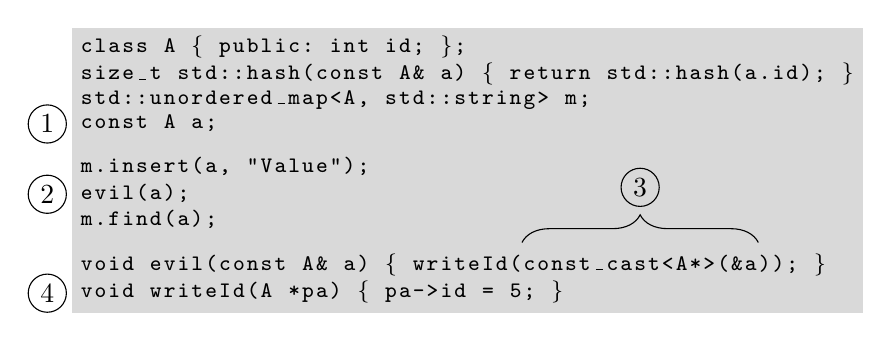
\begin{tikzpicture}
  [node distance=5mm, >=stealth',
  every node/.style={font=\footnotesize},
  every matrix/.style={fill=black!15, inner sep=1mm, row sep=0.5mm,
                        matrix of nodes, nodes in empty cells,
                        minimum height=0.5em, minimum width=.5em,
                        nodes={anchor=base, inner sep=0, font=\ttfamily\footnotesize}}]

  \matrix (snippet) {
c & l & a & s & s &   & A &   & \{ &   & p & u & b & l & i & c & : &   & i & n & t &   & i & d & ; &   & \} & ; &   &   &   &   &   &   &   &   &   &   &   &   &   &   &   &   &   &   &   &   &   &   &   &   &   &   &   &   \\
s & i & z & e & \_ & t &   & s & t & d & : & : & h & a & s & h & ( & c & o & n & s & t &   & A & \& &   & a & ) &   & \{ &   & r & e & t & u & r & n &   & s & t & d & : & : & h & a & s & h & ( & a & . & i & d & ) & ; &   & \} \\
s & t & d & : & : & u & n & o & r & d & e & r & e & d & \_ & m & a & p & < & A & , &   & s & t & d & : & : & s & t & r & i & n & g & > &   & m & ; &   &   &   &   &   &   &   &   &   &   &   &   &   &   &   &   &   &   &   \\
c & o & n & s & t &   & A &   & a & ; &   &   &   &   &   &   &   &   &   &   &   &   &   &   &   &   &   &   &   &   &   &   &   &   &   &   &   &   &   &   &   &   &   &   &   &   &   &   &   &   &   &   &   &   &   &   \\
  &   &   &   &   &   &   &   &   &   &   &   &   &   &   &   &   &   &   &   &   &   &   &   &   &   &   &   &   &   &   &   &   &   &   &   &   &   &   &   &   &   &   &   &   &   &   &   &   &   &   &   &   &   &   &   \\
m & . & i & n & s & e & r & t & ( & a & , &   & " & V & a & l & u & e & " & ) & ; &   &   &   &   &   &   &   &   &   &   &   &   &   &   &   &   &   &   &   &   &   &   &   &   &   &   &   &   &   &   &   &   &   &   &   \\
e & v & i & l & ( & a & ) & ; &   &   &   &   &   &   &   &   &   &   &   &   &   &   &   &   &   &   &   &   &   &   &   &   &   &   &   &   &   &   &   &   &   &   &   &   &   &   &   &   &   &   &   &   &   &   &   &   \\
m & . & f & i & n & d & ( & a & ) & ; &   &   &   &   &   &   &   &   &   &   &   &   &   &   &   &   &   &   &   &   &   &   &   &   &   &   &   &   &   &   &   &   &   &   &   &   &   &   &   &   &   &   &   &   &   &   \\
  &   &   &   &   &   &   &   &   &   &   &   &   &   &   &   &   &   &   &   &   &   &   &   &   &   &   &   &   &   &   &   &   &   &   &   &   &   &   &   &   &   &   &   &   &   &   &   &   &   &   &   &   &   &   &   \\
v & o & i & d &   & e & v & i & l & ( & c & o & n & s & t &   & A & \& &   & a & ) &   & \{ &   & w & r & i & t & e & I & d & ( & c & o & n & s & t & \_ & c & a & s & t & < & A & * & > & ( & \& & a & ) & ) & ; &   & \} &   &   \\
v & o & i & d &   & w & r & i & t & e & I & d & ( & A &   & * & p & a & ) &   & \{ &   & p & a & - & > & i & d &   & = &   & 5 & ; &   & \} &   &   &   &   &   &   &   &   &   &   &   &   &   &   &   &   &   &   &   &   &   \\
  };

  \node [left of=snippet-4-1, circle, draw, font=\normalsize, inner sep=2pt]
        {1};
  \node [left of=snippet-7-1, circle, font=\normalsize, inner sep=2pt, draw]
        {2};
  \draw[decorate, decoration={brace, amplitude=10pt}]
       ($ (snippet-10-33.north west) + (0, 2mm) $)
       -- node[above, yshift=10pt+1mm, circle, font=\normalsize, inner sep=2pt, draw]
       {3}
       ($ (snippet-10-49.north east) + (0, 2mm) $);
  \node [left of=snippet-11-1, circle, font=\normalsize, inner sep=2pt, draw]
        {4};
\end{tikzpicture}

\end{document}
